\documentclass{standalone}
\usepackage{tikz}
\usetikzlibrary{patterns, positioning}
\usetikzlibrary{shapes.misc}
\usepackage[outline]{contour}
\contourlength{1.5pt} 
\usepackage[sfdefault]{ClearSans} %% option 'sfdefault' activates Clear Sans as the default text font
\usepackage[T1]{fontenc}

\begin{document}
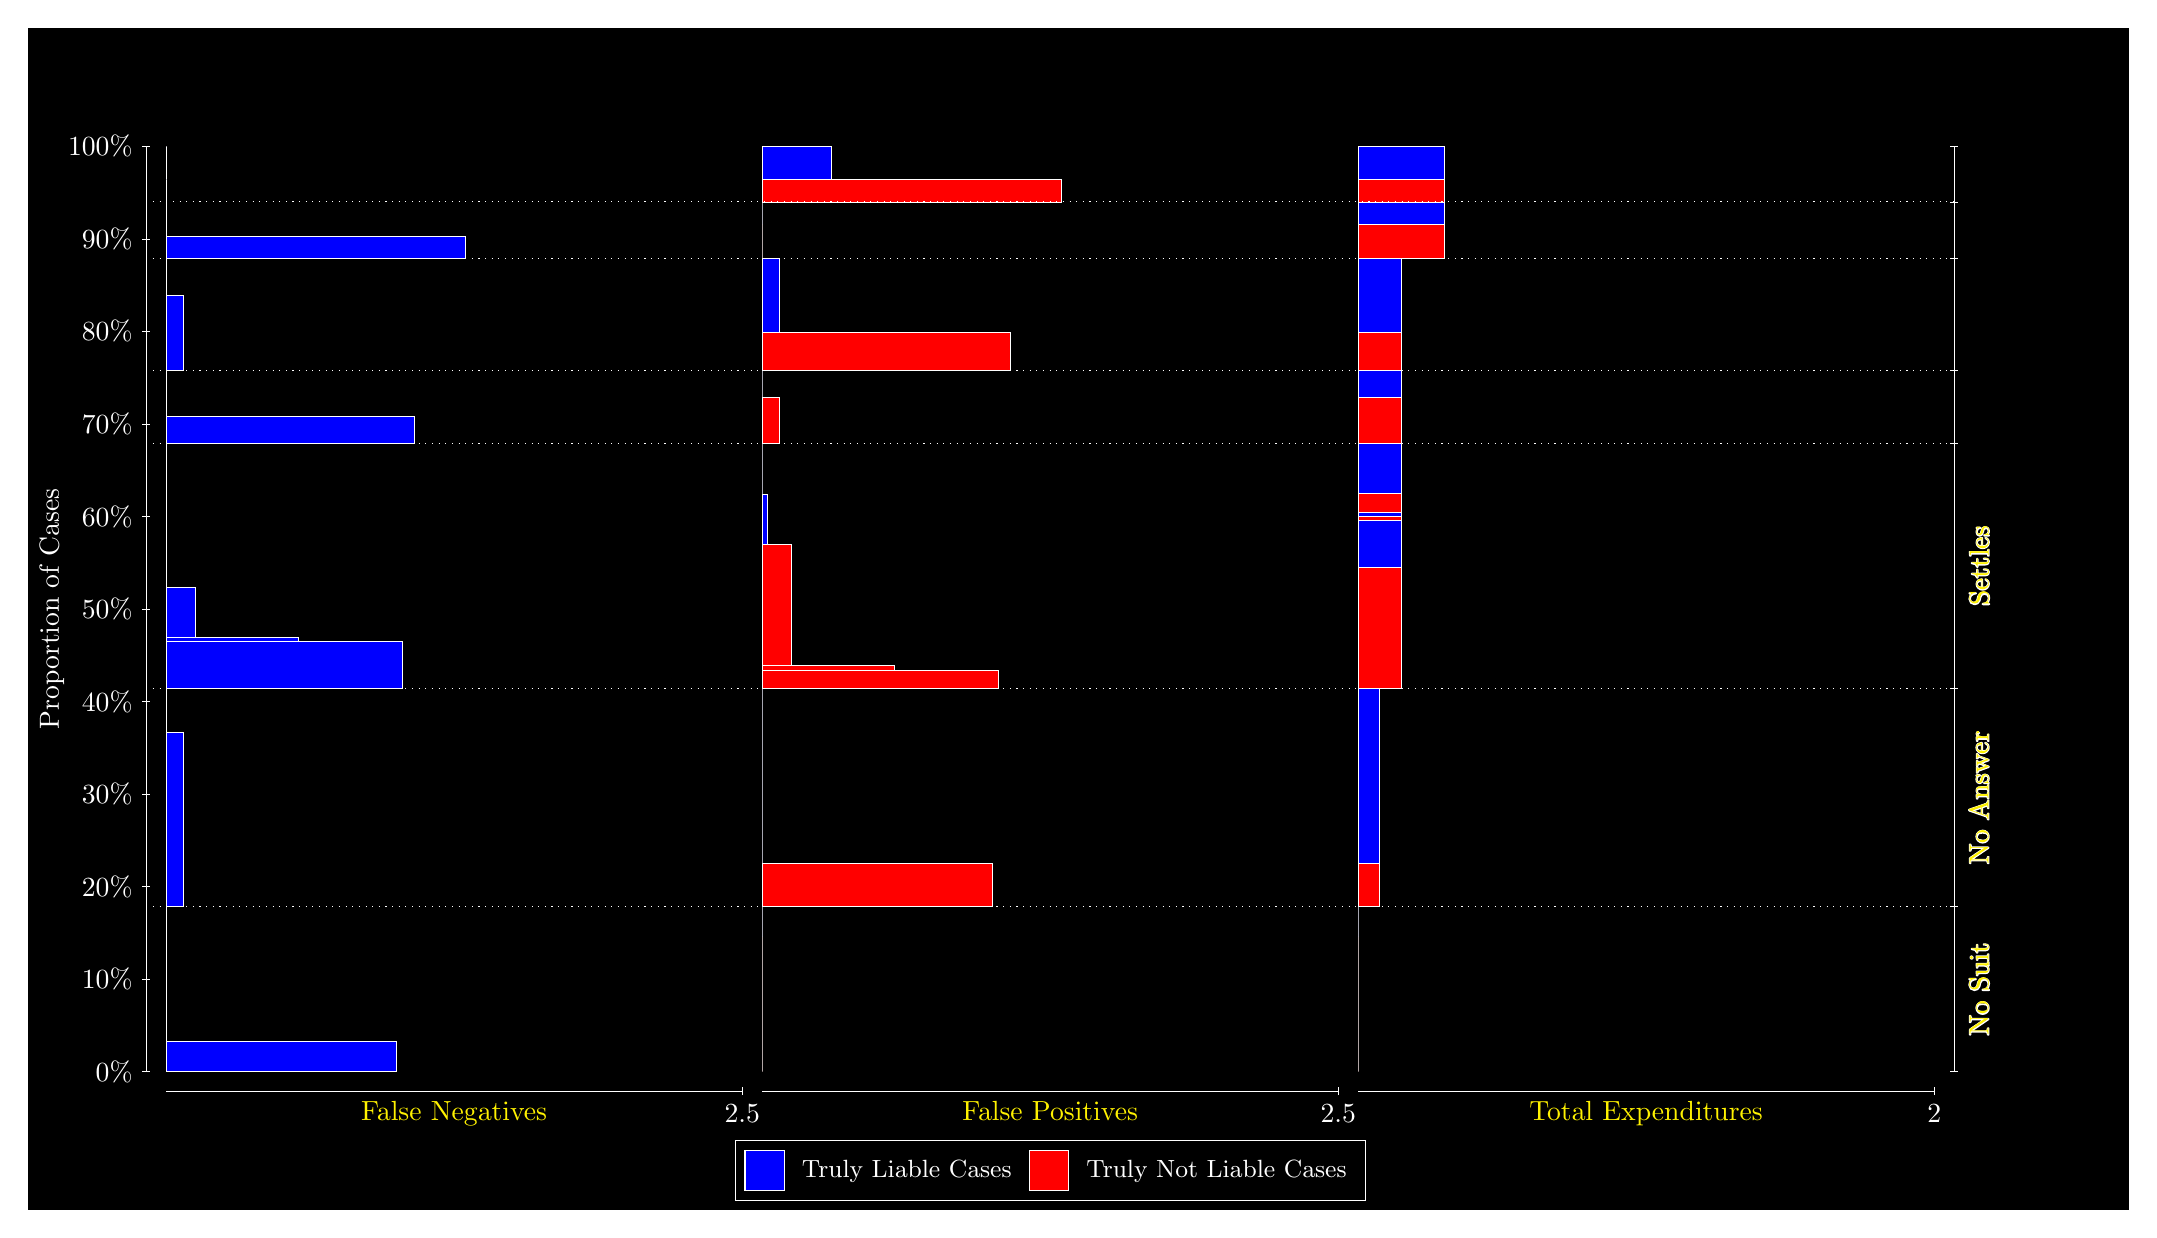
\begin{tikzpicture}
\draw[fill=black] (0,0) rectangle (26.667,15);
\draw[white, very thin] (1.5,1.75) -- (1.5,13.5);
\node[rotate=90, text=white, anchor=center] at (0.3, 7.625) {Proportion of Cases};
\draw[white, very thin] (1.45,1.75) -- (1.55,1.75);
\node[text=white, anchor=east] at (1.45, 1.75) {0\%};
\draw[white, very thin] (1.45,2.925) -- (1.55,2.925);
\node[text=white, anchor=east] at (1.45, 2.925) {10\%};
\draw[white, very thin] (1.45,4.1) -- (1.55,4.1);
\node[text=white, anchor=east] at (1.45, 4.1) {20\%};
\draw[white, very thin] (1.45,5.275) -- (1.55,5.275);
\node[text=white, anchor=east] at (1.45, 5.275) {30\%};
\draw[white, very thin] (1.45,6.45) -- (1.55,6.45);
\node[text=white, anchor=east] at (1.45, 6.45) {40\%};
\draw[white, very thin] (1.45,7.625) -- (1.55,7.625);
\node[text=white, anchor=east] at (1.45, 7.625) {50\%};
\draw[white, very thin] (1.45,8.8) -- (1.55,8.8);
\node[text=white, anchor=east] at (1.45, 8.8) {60\%};
\draw[white, very thin] (1.45,9.975) -- (1.55,9.975);
\node[text=white, anchor=east] at (1.45, 9.975) {70\%};
\draw[white, very thin] (1.45,11.15) -- (1.55,11.15);
\node[text=white, anchor=east] at (1.45, 11.15) {80\%};
\draw[white, very thin] (1.45,12.325) -- (1.55,12.325);
\node[text=white, anchor=east] at (1.45, 12.325) {90\%};
\draw[white, very thin] (1.45,13.5) -- (1.55,13.5);
\node[text=white, anchor=east] at (1.45, 13.5) {100\%};

\draw[white, very thin] (24.457,1.75) -- (24.457,13.5);
\draw[white, very thin] (24.407,1.75) -- (24.507,1.75);
\node[anchor=west] at (24.407, 1.75) {};
\draw[white, very thin] (24.407,3.843) -- (24.507,3.843);
\node[anchor=west] at (24.407, 3.843) {};
\draw[white, very thin] (24.407,6.6136) -- (24.507,6.6136);
\node[anchor=west] at (24.407, 6.6136) {};
\draw[white, very thin] (24.407,9.7283) -- (24.507,9.7283);
\node[anchor=west] at (24.407, 9.7283) {};
\draw[white, very thin] (24.407,10.658) -- (24.507,10.658);
\node[anchor=west] at (24.407, 10.658) {};
\draw[white, very thin] (24.407,12.079) -- (24.507,12.079);
\node[anchor=west] at (24.407, 12.079) {};
\draw[white, very thin] (24.407,12.795) -- (24.507,12.795);
\node[anchor=west] at (24.407, 12.795) {};
\draw[white, very thin] (24.407,13.5) -- (24.507,13.5);
\node[anchor=west] at (24.407, 13.5) {};

\draw[white, very thin, fill=blue] (1.75,1.75) rectangle (4.6775,2.1326);
\draw[white, very thin, fill=red] (1.75,2.1326) rectangle (1.75,3.843);
\draw[white, very thin, fill=blue] (1.75,3.843) rectangle (1.9696,6.0591);
\draw[white, very thin, fill=red] (1.75,6.0591) rectangle (1.75,6.6136);
\draw[white, very thin, fill=blue] (1.75,6.6136) rectangle (4.7507,7.2085);
\draw[white, very thin, fill=blue] (1.75,7.2085) rectangle (3.4333,7.2606);
\draw[white, very thin, fill=blue] (1.75,7.2606) rectangle (2.1159,7.9001);
\draw[white, very thin, fill=red] (1.75,7.9001) rectangle (1.75,9.7283);
\draw[white, very thin, fill=blue] (1.75,9.7283) rectangle (4.8971,10.068);
\draw[white, very thin, fill=red] (1.75,10.068) rectangle (1.75,10.658);
\draw[white, very thin, fill=blue] (1.75,10.658) rectangle (1.9696,11.602);
\draw[white, very thin, fill=red] (1.75,11.602) rectangle (1.75,12.079);
\draw[white, very thin, fill=blue] (1.75,12.079) rectangle (5.5558,12.363);
\draw[white, very thin, fill=red] (1.75,12.363) rectangle (1.75,12.795);
\draw[white, very thin, fill=red] (1.75,12.795) rectangle (1.75,13.077);
\draw[white, very thin, fill=blue] (1.75,13.077) rectangle (1.75,13.5);
\draw[white, very thin, fill=red] (9.3189,1.75) rectangle (9.3189,3.4605);
\draw[white, very thin, fill=blue] (9.3189,3.4605) rectangle (9.3189,3.843);
\draw[white, very thin, fill=red] (9.3189,3.843) rectangle (12.246,4.3976);
\draw[white, very thin, fill=blue] (9.3189,4.3976) rectangle (9.3189,6.6136);
\draw[white, very thin, fill=red] (9.3189,6.6136) rectangle (12.32,6.8511);
\draw[white, very thin, fill=red] (9.3189,6.8511) rectangle (11.002,6.9032);
\draw[white, very thin, fill=red] (9.3189,6.9032) rectangle (9.6848,8.4418);
\draw[white, very thin, fill=blue] (9.3189,8.4418) rectangle (9.3921,9.0813);
\draw[white, very thin, fill=blue] (9.3189,9.0813) rectangle (9.3189,9.7283);
\draw[white, very thin, fill=red] (9.3189,9.7283) rectangle (9.5384,10.319);
\draw[white, very thin, fill=blue] (9.3189,10.319) rectangle (9.3189,10.658);
\draw[white, very thin, fill=red] (9.3189,10.658) rectangle (12.466,11.135);
\draw[white, very thin, fill=blue] (9.3189,11.135) rectangle (9.5384,12.079);
\draw[white, very thin, fill=red] (9.3189,12.079) rectangle (9.3189,12.512);
\draw[white, very thin, fill=blue] (9.3189,12.512) rectangle (9.3189,12.795);
\draw[white, very thin, fill=red] (9.3189,12.795) rectangle (13.125,13.077);
\draw[white, very thin, fill=blue] (9.3189,13.077) rectangle (10.197,13.5);
\draw[white, very thin, fill=red] (16.888,1.75) rectangle (16.888,3.4605);
\draw[white, very thin, fill=blue] (16.888,3.4605) rectangle (16.888,3.843);
\draw[white, very thin, fill=red] (16.888,3.843) rectangle (17.162,4.3976);
\draw[white, very thin, fill=blue] (16.888,4.3976) rectangle (17.162,6.6136);
\draw[white, very thin, fill=red] (16.888,6.6136) rectangle (17.437,8.1523);
\draw[white, very thin, fill=blue] (16.888,8.1523) rectangle (17.437,8.7472);
\draw[white, very thin, fill=red] (16.888,8.7472) rectangle (17.437,8.7992);
\draw[white, very thin, fill=blue] (16.888,8.7992) rectangle (17.437,8.8513);
\draw[white, very thin, fill=red] (16.888,8.8513) rectangle (17.437,9.0888);
\draw[white, very thin, fill=blue] (16.888,9.0888) rectangle (17.437,9.7283);
\draw[white, very thin, fill=red] (16.888,9.7283) rectangle (17.437,10.319);
\draw[white, very thin, fill=blue] (16.888,10.319) rectangle (17.437,10.658);
\draw[white, very thin, fill=red] (16.888,10.658) rectangle (17.437,11.135);
\draw[white, very thin, fill=blue] (16.888,11.135) rectangle (17.437,12.079);
\draw[white, very thin, fill=red] (16.888,12.079) rectangle (17.986,12.512);
\draw[white, very thin, fill=blue] (16.888,12.512) rectangle (17.986,12.795);
\draw[white, very thin, fill=red] (16.888,12.795) rectangle (17.986,13.077);
\draw[white, very thin, fill=blue] (16.888,13.077) rectangle (17.986,13.5);
\draw[white, dotted] (1.5,3.843) -- (24.457,3.843);
\draw[white, dotted] (1.5,6.6136) -- (24.457,6.6136);
\draw[white, dotted] (1.5,9.7283) -- (24.457,9.7283);
\draw[white, dotted] (1.5,10.658) -- (24.457,10.658);
\draw[white, dotted] (1.5,12.079) -- (24.457,12.079);
\draw[white, dotted] (1.5,12.795) -- (24.457,12.795);
\draw[white, very thin] (1.75,1.5) -- (9.0689,1.5);
\node[text=yellow, anchor=north] at (5.4094, 1.5) {False Negatives};
\draw[white, very thin] (9.0689,1.45) -- (9.0689,1.55);
\node[text=white, anchor=north] at (9.0689, 1.45) {2.5};

\draw[white, very thin] (9.3189,1.5) -- (16.638,1.5);
\node[text=yellow, anchor=north] at (12.978, 1.5) {False Positives};
\draw[white, very thin] (16.638,1.45) -- (16.638,1.55);
\node[text=white, anchor=north] at (16.638, 1.45) {2.5};

\draw[white, very thin] (16.888,1.5) -- (24.207,1.5);
\node[text=yellow, anchor=north] at (20.547, 1.5) {Total Expenditures};
\draw[white, very thin] (24.207,1.45) -- (24.207,1.55);
\node[text=white, anchor=north] at (24.207, 1.45) {2};

\node[text=yellow, centered, rotate=90] at (24.777, 2.7965) {\contour{white}{No Suit}};
\node[text=yellow, centered, rotate=90] at (24.777, 5.2283) {\contour{white}{No Answer}};
\node[text=yellow, centered, rotate=90] at (24.777, 8.171) {\contour{white}{Settles}};





\draw (12.978300999999998,1.5) node[draw=none] (baseCoordinate) {};
\begin{scope}[align=center]
        \matrix[scale=0.5, draw=white, below=0.5cm of baseCoordinate, nodes={draw}, column sep=0.1cm]{
            \node[rectangle, draw, minimum width=0.5cm, minimum height=0.5cm, fill=blue] {}; &
            \node[draw=none, font=\small, text=white] (B) {Truly Liable Cases}; &
            \node[rectangle, draw, minimum width=0.5cm, minimum height=0.5cm, fill=red] {}; &
            \node[draw=none, font=\small, text=white] (B) {Truly Not Liable Cases}; \\
            };
\end{scope}

\end{tikzpicture}
\end{document}